\documentclass[a4paper, 12pt, dvipdfmx, uplatex]{jsreport}
% \usepackage[top=30truemm, bottom=30truemm, left=25truemm, right=25truemm]{geometry} % 余白設定
% \usepackage[dvipdfmx]{pdflscape}


\usepackage{url}
% \usepackage{moreverb}

\usepackage{listings,jvlisting} %ソースコード埋め込み
\lstset{
  basicstyle={\ttfamily},
  identifierstyle={\small},
  commentstyle={\smallitshape},
  keywordstyle={\small\bfseries},
  ndkeywordstyle={\small},
  stringstyle={\small\ttfamily},
  frame={tb},
  breaklines=true,
  columns=[l]{fullflexible},
  numbers=left,
  xrightmargin=0zw,
  xleftmargin=3zw,
  numberstyle={\scriptsize},
  stepnumber=1,
  numbersep=1zw,
  lineskip=-0.5ex
}
\makeatletter
\def\lst@lettertrue{\let\lst@ifletter\iffalse}
\makeatother
\renewcommand{\lstlistingname}{プログラム}

% ================ Quick Half Quad Text bgn =========================
\newcommand{\hqq}[1]{\ \mathtt{#1}\ }
\newcommand{\hqif}{\hqq{if}}
\newcommand{\hqthen}{\hqq{then}}
\newcommand{\hqelse}{\hqq{else}}
\newcommand{\hqwhile}{\hqq{while}}
\newcommand{\hqdo}{\hqq{do}}
\newcommand{\hqskip}{\hqq{skip}}

\newcommand{\hqql}[1]{\ \mathtt{#1}}
\newcommand{\hqlif}{\hqql{if}}
\newcommand{\hqlthen}{\hqql{then}}
\newcommand{\hqlelse}{\hqql{else}}
\newcommand{\hqlwhile}{\hqql{while}}
\newcommand{\hqldo}{\hqql{do}}
\newcommand{\hqlskip}{\hqql{skip}}

\newcommand{\hqqr}[1]{\mathtt{#1}\ }
\newcommand{\hqrif}{\hqqr{if}}
\newcommand{\hqrthen}{\hqqr{then}}
\newcommand{\hqrelse}{\hqqr{else}}
\newcommand{\hqrwhile}{\hqqr{while}}
\newcommand{\hqrdo}{\hqqr{do}}
\newcommand{\hqrskip}{\hqqr{skip}}

\newcommand{\nhqq}[1]{\mathtt{#1}}
\newcommand{\nhqskip}{\nhqq{skip}}
\newcommand{\x}{\nhqq{x}}
\newcommand{\y}{\nhqq{y}}
\newcommand{\z}{\nhqq{z}}
% ================ Quick Half Quad Text end =========================

%定理環境
\theoremstyle{definition}
\newtheorem{dfn}{定義}
\newtheorem{thm}{定理}
\newtheorem{lemma}{補題}

\usepackage[dvipdfmx]{graphicx} % グラフを入れるのに必要
\usepackage[dvipdfmx]{color} % グラフを入れるのに必要
\usepackage{fancyhdr} % ページ数指定に必要
\usepackage{lastpage} % 同上
\usepackage{multirow} % 表で縦複数行にまたがるセルを作るのに必要
\usepackage{amsmath} % 一部の数学記号や数学的表現をするために必要
\usepackage{autobreak}
\usepackage{amsfonts} % 同上
\usepackage{amssymb} % 同上
\usepackage{bm} % 太字に必要
\usepackage{siunitx} % SI単位系の斜体を直す
\usepackage{here}
\usepackage{wrapfig}
\usepackage{breqn} % dmath でいい感じに数式を折り返してくれる
% \usepackage{pdfpages} % pdf を挿入できる
% \usepackage{slashbox} % 表に斜め線を入れるやつ このtexファイルがあるディレクトリと同じところにslashbox.styを置くとかする必要がある。

\usepackage{breqn}
\usepackage{wrapfig}
\usepackage{physics}
\usepackage{mathrsfs}
\usepackage{mathtools}
\usepackage{bussproofs}

\usepackage{lscape}

% \newcommand{\unit}[1]{\mathrm{[#1]}} % 単位の括弧[]
\newcommand{\tup}[1]{\left\langle{#1}\right\rangle}

% % タイトルを明朝体で書く
% % \titleformat* は \titleformat を短く書く方法. 
\usepackage{titlesec}
% \titleformat*{\section}{\Large\bfseries}
% \titleformat*{\section}{\large\bfseries}
% \titleformat*{\subsection}{\large\bfseries}
% \titleformat*{\subsection}{\normalsize\bfseries}
% \titleformat*{\subsubsection}{\normalsize\bfseries}

% ページの右下にページ数を記載するスタイル
% \fancypagestyle{mypagestyle}{
%   \lhead{}
%   \rhead{}
%   \fancyfoot[C]{}
%   \fancyfoot[R]{p.\thepage/\pageref{LastPage}}
%   \renewcommand{\headrulewidth}{0.0pt}
% }

% ページスタイルを適用
% \pagestyle{mypagestyle}

% \maketitle コマンドをdocument内に入れることで, タイトルページが自動生成される
% \title{プログラミング言語特論 \quad 課題1}
% \author{1W192258-2 \quad 富家功一朗}

% \makeatletter
%   \renewcommand{\thesubsection}{\arabic{section}.\arabic{subsection}}
%   \@addtoreset{subsection}{section}
% \makeatother

% \renewcommand{\thesection}{\textbf{[\arabic{section}]}}
% \renewcommand{\thesubsection}{(\alph{subsection})}

% 式番号を章.式番 の形式にさせる
%  \makeatletter
%    \renewcommand{\theequation}{\arabic{section}.\arabic{equation}}
%    \@addtoreset{equation}{section}
%  \makeatother

% 表番号も
%  \makeatletter
%    \renewcommand{\thetable}{\arabic{section}.\arabic{table}}
%    \@addtoreset{table}{section}
%  \makeatother

% 図番号も
%  \makeatletter
%    \renewcommand{\thefigure}{\arabic{section}.\arabic{figure}}
%    \@addtoreset{figure}{section}
%  \makeatother

% ソースコード番号も
%  \makeatletter      
%       \AtBeginDocument{                       
%           \renewcommand*{\thelstlisting}{\arabic{section}.\arabic{lstlisting}}          
%           \@addtoreset{lstlisting}{section}                    
%       }            
%  \makeatother

% 参考文献の番号を 1) にする
% \makeatletter
%   \def\@biblabel#1{#1)}
% \makeatletter

% 図の入れ方
% \begin{figure}[H] % h...hereの意
%   \centering
%   \includegraphics[width=13cm]{kairo.png}
%   \caption{キャプション名\label{ラベル名}}
% \end{figure}

% 回り込む図
% \begin{wrapfigure}[13]{r}{5cm}
%   \centering
%   \includegraphics[width=5cm]{img/schematics.png}
%   \vspace*{-\intextsep}
%   \caption{システムの模式図\label{schematics}}
% \end{wrapfigure}

% 表の入れ方
% \begin{table}[H]
%   \centering
%   \caption{キャプション名\label{ラベル名}}
%   \begin{tabular}{c|c|c|c} \hline \hline
%     抵抗名 &$\zeta$ &$\psi$ & $g :\ \mathrm{dB}$ \\\hline
%     R1&$0.0500$ &$ 0.997 $ & $20.0$\\\hline
%     R3 & $0.500$ &$0.707$ & $2.32$ \\\hline
%   \end{tabular}
% \end{table}

% ソースコードの埋め込み方
% \begin{lstlisting}[caption=name,label=number]
% \end{lstlisting}

% pdf 挿入の仕方
% \includepdf[pages=-]{pdfs/reviews.pdf}
% \includepdf[pages=3]{pdfs/FrontCovers.pdf}
% \includepdf[pages=2-]{pdfs/report1.pdf}

% prooftree
% \begin{prooftree}
%   \AxiomC{}
%   \RightLabel{$\overrightarrow{\mathtt{var}}$}
%   \UnaryInfC{$\tup{x, s}\to \tup{1, s}$}
%   \RightLabel{$\overrightarrow{\mathtt{op1}}$}
%   \UnaryInfC{$\tup{x\leq y, s}\to \tup{1\leq y, s}$}
%   \RightLabel{$\overrightarrow{\mathtt{if1}}$}
%   \UnaryInfC{$\tup{\hqrif x \leq y \hqthen C_1 \hqelse \nhqskip, s}\to \tup{\hqrif 1 \leq y \hqthen C_1 \hqelse \nhqskip, s}$}
%   \RightLabel{$\overrightarrow{\mathtt{seq1}}$}
%   \UnaryInfC{$\tup{(\hqrif x \leq y \hqthen C_1 \hqelse \nhqskip );(z \coloneqq 3; C_2), s}\to \tup{(\hqrif 1 \leq y \hqthen C_1 \hqelse \nhqskip );(z \coloneqq3; C_2), s}$}
% \end{prooftree}

\setcounter{tocdepth}{3}

\title{ReDoS脆弱な正規表現の修正}
\author{情報理工学科 寺内研究室所属 富家功一朗}
\date{2023年1月31日}

\begin{document}
\chapter{既存研究}


\section{ReDoS脆弱性}
文字列のパターンマッチングにかなり時間がかかってしまうような正規表現が存在することが知られている.そのような正規表現をReDoS(regular expression denial-of-service)脆弱な正規表現と呼ぶ.本節ではまず文字列のパターンマッチングはどのようなアルゴリズムで行われているかを紹介し,その次に正規表現の脆弱性について定義する.

\subsection{バックトラック探索}
大抵のプログラミング言語が正規表現ライブラリを提供している.そのうち多くの正規表現ライブラリはバックトラック探索アルゴリズムを用いて文字列のパターンマッチングを行っている.このアルゴリズムにおいてバックトラックとはどのようなものなのか,それを\cite{javascript}の論文で紹介されていた例を用いて説明する.バックトラック探索アルゴリズムの詳細は\cite{java}を参照されたい(プログラミング言語Javaにおける,バックトラック探索アルゴリズムを用いた文字列パターンマッチングについて述べられている).

$a^*a^*b$という正規表現について考える.この正規表現と等価なNFAは以下のように作成できる(\cite{javascript}より引用).

\begin{figure}[H] % h...hereの意
  \centering
  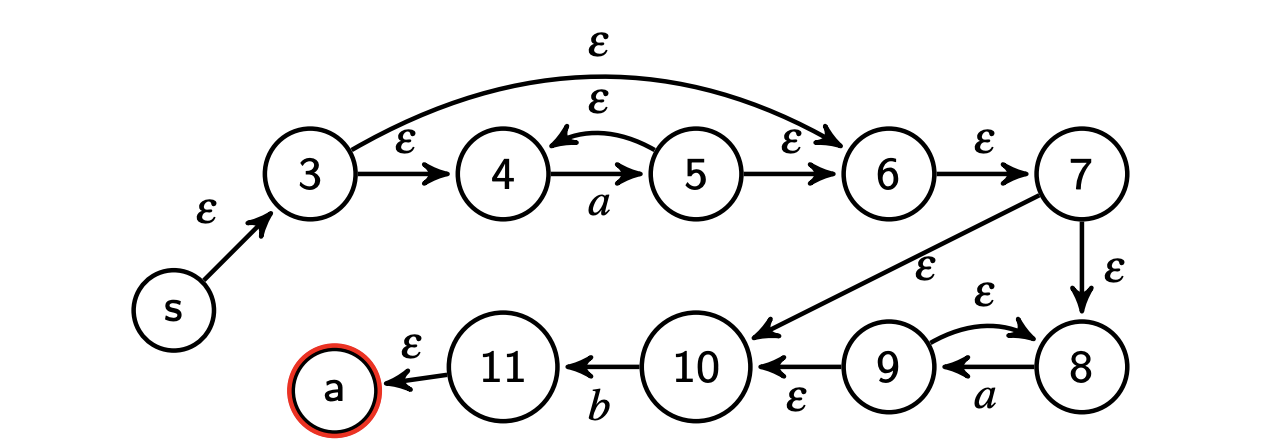
\includegraphics[width=0.8\linewidth]{../figures/a*a*b.png}
  \caption{正規表現$a^*a^*b$と等価なNFA\label{ラベル名}}
\end{figure}


このNFAに$aaa$という文字列を入力として与える(なお,$aaa$は受理されない).

まず,初期状態$s$から遷移できるところまで進む.今回の例では初期状態$s$から$a$という文字を2つ消費した後の状態10までは遷移できる.これをパスとして表すと以下のようになる.
\begin{equation}
  (s,\varepsilon,3),(3,\varepsilon,4),(4,a,5),(5,\varepsilon,6),(6,\varepsilon,7),(7,\varepsilon,8),(8,a,9),(9,\varepsilon,10)\label{path1}
\end{equation}
他にも以下のようなパスが存在する.
\begin{equation*}
  (s,\varepsilon,3),(3,\varepsilon,4),(4,a,5),(5,\varepsilon,4),(4,a,5),(5,\varepsilon,6),(6,\varepsilon,7),(7,\varepsilon,10)
\end{equation*}
\begin{equation*}
  (s,\varepsilon,3),(3,\varepsilon,6),(6,\varepsilon,7),(7,\varepsilon,8),(8,a,9),(9,\varepsilon,8),(8,a,9),(9,\varepsilon,10)
\end{equation*}
しかし,状態10から先へは文字$b$がなければ進めない.このような状況に陥った際,1手前に戻る,すなわちバックトラックが行われる.具体的に言えば,(\ref{path1})の探索パスで言えば状態10から進めないことが分かったので状態9に戻ってやり直すということである.状態9に戻って,残りの文字$a$を読み取った上で状態$a$にたどりつけるようなパスを探すが存在しないので,またバックトラックする.このように文字列のパターンマッチングではバックトラックを繰り返し行うことが多々ある.バックトラックの回数が文字列のパターンマッチングの実行時間に大きな影響を与える.


\subsection{ReDoS脆弱性の定式化}
ReDoS脆弱性の定式化を行う.W\"{u}stholzらの研究\cite{vul_detect}では,超脆弱なNFAと脆弱なNFAの2種類の定義が紹介されていた.なお,本節でのNFAは$\varepsilon$遷移なしNFAである.

\subsubsection{超脆弱なNFA}
まず,超脆弱な($\varepsilon$遷移なし)NFAについて定式化する.

\subsubsection{脆弱なNFA}
次に,脆弱な($\varepsilon$遷移なし)NFAについて定式化する.
\begin{dfn}[脆弱なNFA]
  NFA $\mathcal{A}=(Q,\Sigma,\Delta,q_0,F)$が脆弱であることは$\mathcal{A}$のパスを走査するようなバックトラック探索アルゴリズムMATCHが存在し,MATCHの最悪ケースの複雑さが入力文字列の長さに対して最低でも2次関数的になることと同値である.
\end{dfn}

\begin{thm}\label{thm1}
  NFA $\mathcal{A}$が脆弱であることは以下の条件を満たすような2つのピボット状態$q\in Q$と3つのパス$\pi_1,\pi_2,\pi_3$(ただし,$\pi_1 \neq \pi_2$)が存在することと同値である.
    \begin{enumerate}
      \item $\pi_1$は$q$で始まり,$q$で終わる.
      \item $\pi_2$は$q$で始まり,$q'$で終わる.
      \item $\pi_3$は$q'$で始まり,$q'$で終わる.
      \item labels($\pi_1$)=label($\pi_2$)=label($\pi_3$).
      \item $q_0$から$q$へのパス$\pi_p$が存在する.
      \item $q'$から状態$q_r \notin F$へのパス$\pi_s$が存在する.
    \end{enumerate}
\end{thm}
証明については\cite{vul_detect}を参照されたい.

上記の定理を直感的に表した図を以下に示す(\cite{vul_detect}より引用).
\begin{figure}[H] % h...hereの意
  \centering
  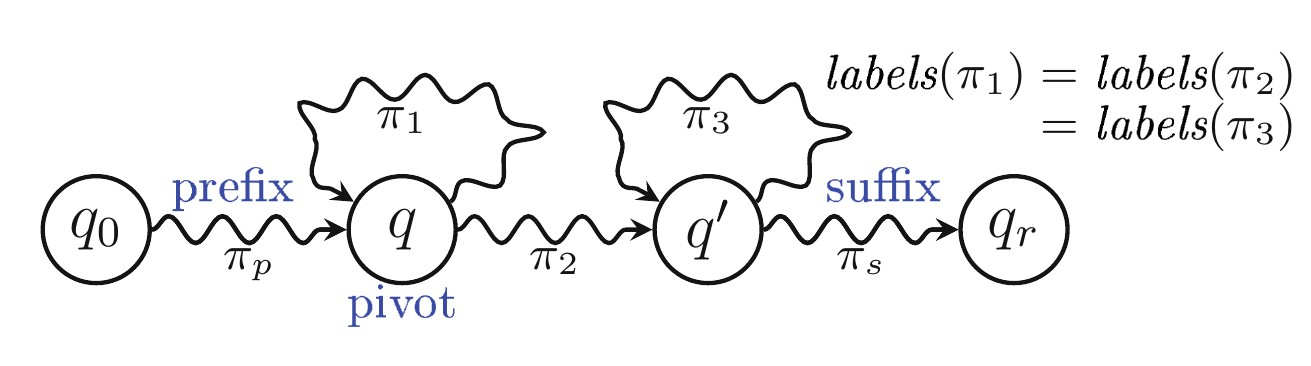
\includegraphics[width=\linewidth]{../figures/vul.jpg}
  \caption{脆弱なNFAの一般的なパターン\label{vul_nfa}}
\end{figure}

定理\ref{thm1}の性質を満たすNFAが超線形的な動作を引き起こす理由を考える.

$s_0\cdot s^k\cdot s_1$という形の攻撃文字列を考える.$s_0$が攻撃文字列のプレフィックスlabels($\pi_p$),$s_1$が攻撃文字列のサフィックスlabels($\pi_s$),$s$が攻撃文字列のコアlabels($\pi_1$)である.そして,$s_0\cdot s^k\cdot s_1$が拒絶される実行パスが存在する($\pi_p \cdot \pi_1^k \cdot \pi_s$など).$T_q(k)$は$q$から走査を開始し,文字列$s^k\cdot s_1$を拒絶するまでの実行時間(文字列$s$を読むのに1単位の時間がかかるとする)を表すものとすると,以下のような漸化式が作れる.

\begin{align}
  T_q(k)=(1+T_q(k-1))+(1+T_{q'}(k-1))\label{tq}
\end{align}

式(\ref{tq})の右辺を詳しくみると,文字列$s$は以下の2パターンの方法で処理されることが分かる.
\begin{enumerate}
  \item パス$\pi_1$を通って$q$に戻る場合,$s$が1単位分処理される.現状$q$にいるため,$T_q(k-1)$単位分の処理が残る.
  \item パス$\pi_2$を通って$q'$へ行く場合,$s$が1単位分処理される.現状$q'$にいるため,$T_{q'}(k-1)$単位分の処理が残る.
\end{enumerate}

ここで,$T_{q'}(k)$の下界は$k$である.なぜなら,パス$\pi_3^k \pi_s$は明らかに拒絶状態$q_r$に到達できるからである.このことから,
\begin{align*}
  T_q(k)\geq T_q(k-1)+k+1
\end{align*}
従って,NFA $\mathcal{A}$において文字列$s_0\cdot s^k\cdot s_1$のパターンマッチングには最低でも$k^2$オーダーの時間がかかる.

脆弱なNFAの例を以下に示す(\cite{vul_detect}より引用).
\begin{figure}[H] % h...hereの意
  \centering
  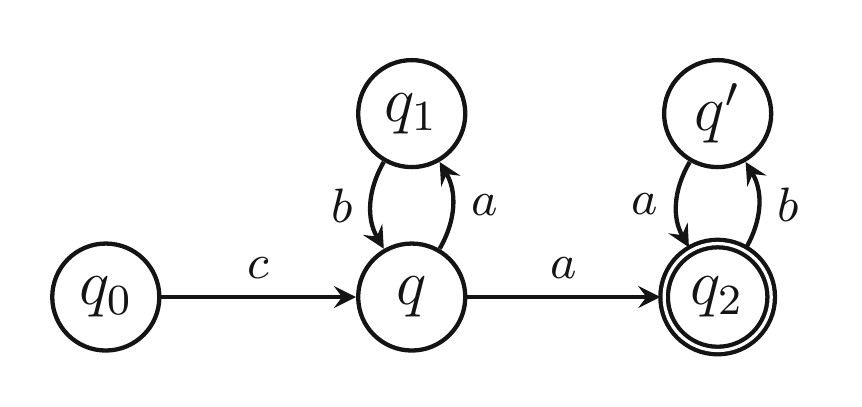
\includegraphics[width=0.75\linewidth]{../figures/vul_ex.jpg}
  \caption{脆弱なNFAの例\label{vul_ex}}
\end{figure}

$\pi_1$が$(q,a,q_1),(q_1,b,q)$,$\pi_2$が$(q,a,q_2),(q_2,b,q')$,$\pi_3$が$(q,a,q_2),(q_2,b,q)$とすると,定理\ref{thm1}より図\ref{vul_ex}は脆弱である.


% コピペ
% 直感的に


\section{REMEDY}
プログラマーがReDoS脆弱な正規表現を発見したとして,その正規表現をどのように扱いたいだろうか.その正規表現を非脆弱化したいと考える人が多いのではないだろうか.そこで,本章では脆弱な正規表現を非脆弱なものへと変換するツールREMEDY\cite{remedy}を紹介する.

REMEDYは例を用いて正規表現を修正するprogramming-by-example(PBE)という手法を用いていて,正規表現の修正手法として多くの研究で注目されている.修正したい正規表現とその正規表現に受理されてほしい文字列例(positive example,正例)と受理されてほしくない文字列例(negative example,負例)を用いて正規表現を合成するというのがPBEを用いた正規表現修正のアプローチである.REMEDYは入力として正規表現,positive example,negative exampleを受けとり,出力として以下の性質を満たすような正規表現を返す.
\begin{enumerate}
  \item 入力として与えられたpositive example,negative exampleが正しく分類されている(positive exampleは受理され,negative exampleは受理されない)
  \item real-world strong 1-unambuiguity(RWS1U)
  \item 入力として与えられた正規表現に構文的に近い
\end{enumerate}
real-world strong 1-unambuiguity(RWS1U)を満たせば正規表現が非脆弱であることが保証される(今回扱う正規表現は純粋なものなのでS1Uを満たすだけでも非脆弱であることが保証される).入力として与えられた正規表現に構文的に近いというのは入力の正規表現$r$と出力の正規表現$r'$の編集距離が最小になるということである.詳細に言うと,正規表現を構文木としてみなしたとき,編集前の部分木の節点の個数と編集後の部分木の節点の個数の和が最小になるということである.

% abstract,intro抜粋





% REMEDYがどういうものか
% S1Uとか







\bibliography{main}
\bibliographystyle{junsrt}


\end{document}